\chapter{T-04: Métrica oficial y trazabilidad}

\section{Problema}

Coexistían múltiples cifras de F1-macro para mBERT (0.7862 en auditoría, 0.778 en redondeos legacy, 0.7715 solo validación) sin una regla única de selección del checkpoint.

\section{Regla oficial}

\begin{itemize}[noitemsep]
  \item Checkpoint: mejor validación (\texttt{checkpoint-1072}).
  \item Una sola evaluación sobre \texttt{test.csv} ($n=460$).
  \item Metadatos en \texttt{mbert\_official\_run.json} (run\_id, commit, hash del test, semilla).
\end{itemize}

\section{Trazabilidad}

\begin{table}[H]
  \centering
  \caption{Inventario F1-macro mBERT}
  \label{tab:traceability}
  \begin{tabular}{lclll}
\toprule
F1-macro & Estado & Fuente & Checkpoint & Split \\
\midrule
0.7777 & Oficial & reports/metrics/mbert\_test\_metrics.csv & checkpoint-1072 & test \\
0.7780 & Mismo run (redondeo) & reports/latex/chapters (histórico) & checkpoint-1072 & test \\
0.7862 & No reproducible & Informe\_Auditoria\_de\_Modelos.docx (Tabla 7) & desconocido & test \\
0.7715 & Solo validación & models/mbert-sv/train\_metrics.json / val & checkpoint-1072 & val \\
\bottomrule
\end{tabular}

\end{table}

\section{Métricas globales oficiales}

\begin{table}[H]
  \centering
  \caption{Métricas globales mBERT (test oficial)}
  \label{tab:mbert-global}
  \begin{tabular}{lc}
\toprule
Métrica & Valor \\
\midrule
Accuracy & 0.7826 \\
Balanced accuracy & 0.7757 \\
F1-macro & 0.7777 \\
F1-weighted & 0.7829 \\
MCC & 0.7036 \\
QWK & 0.7362 \\
Kappa lineal & 0.7182 \\
Ordinal MAE & 0.3239 \\
Ordinal RMSE & 0.7561 \\
Errores grandes (\%) & 8.9130 \\
ROC-AUC OVR & 0.9222 \\
Log-loss & 0.8721 \\
ECE & 0.1569 \\
Brier macro & 0.0940 \\
F1 bootstrap lo & 0.7358 \\
F1 bootstrap hi & 0.8144 \\
\bottomrule
\end{tabular}

\end{table}

\begin{figure}[H]
  \centering
  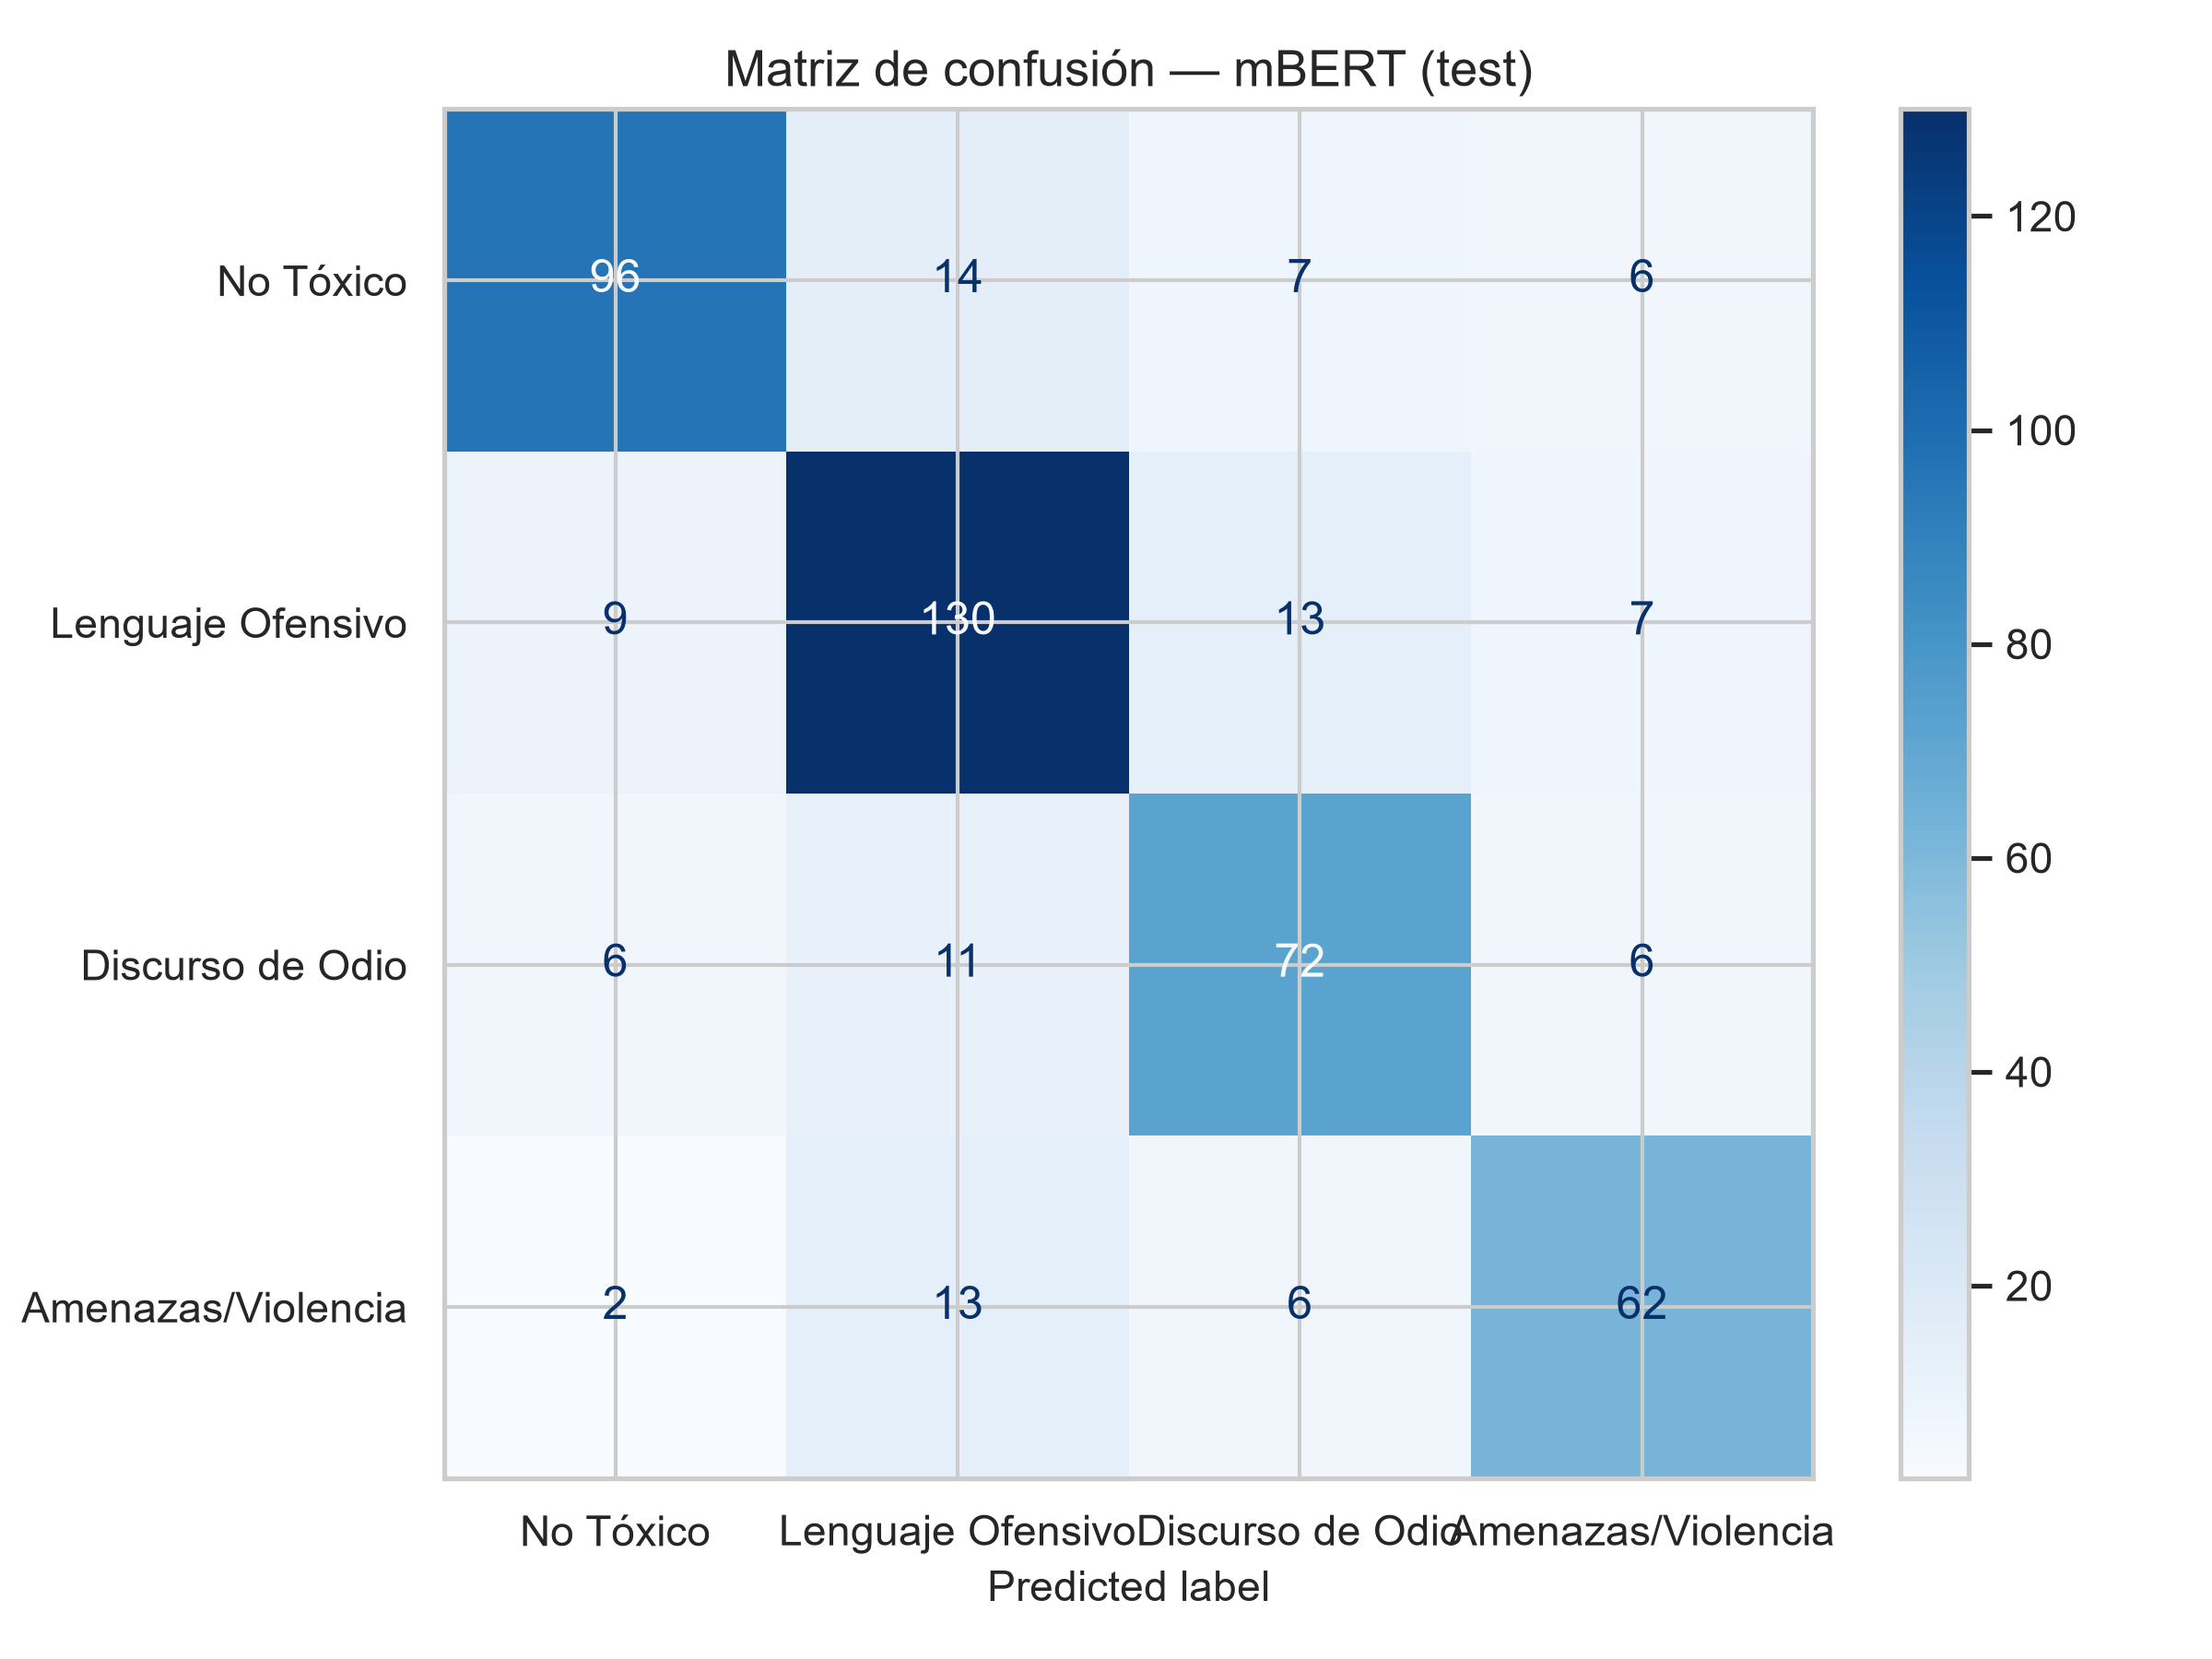
\includegraphics[width=0.75\textwidth]{04_confusion_matrix.png}
  \caption{Matriz de confusión mBERT (test, $n=460$)}
  \label{fig:confusion}
\end{figure}

\textbf{Criterio de cierre:} toda cifra publicada proviene de \texttt{mbert\_test\_metrics.csv}; 0.7862 marcado como no reproducible.
